\subsection{OSN 24 Линейные методы в машинном обучении: линейная и гребневая регрессии, метод опорных векторов. Регуляризация в линейных методах.}

\subsubsection{Линейная регрессия}
Метод определения целевых значений по формуле $a(X_1, ..., X_n) = w_0 + w_1X_1 + ... + w_nX_n$ называется «линейной регрессией». Здесь $X_1, ..., X_n$ - значения признаков объекта.

Одномерный случай $a(X_1) = w_0 + w_1X_1$:

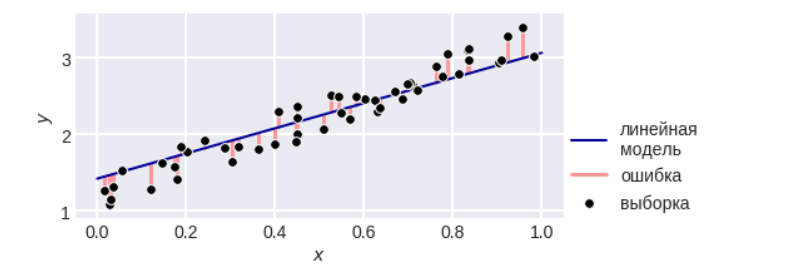
\includegraphics[scale=0.4]{pics/ml2_lin1.png}

Предполагая что целевые значения задаются линейно представим следующую систему:
\begin{equation*}
 \begin{cases}
   w_0 + w_1x_1 = y_1,
   \\
   ...
   \\
   w_0 + w_1x_m = y_m.
 \end{cases}
\end{equation*}

Но вряд ли система решается точно (она может быть несовместна, особенно при довольно большом объёме обучающей выборки m).
Формулы для "невязки" (отклонения/ошибок):
\begin{equation*}
 \begin{cases}
   e_1 = y_1 - w_0 + w_1x_1,
   \\
   ...
   \\
   e_m = y_m - w_0 + w_1x_m.
 \end{cases}
\end{equation*}
Задача обучения линейной регрессии - задача минимизации суммы квадратов
отклонений:
$e_1^2 + ... + e_m^2 \rightarrow min$

Или же задача минимизации эмпирического риска по параметрам $w=(w_0, w_1)$:

$L(w) = \sum\limits_{i=1}^m (y_i - a_w(x_i))^2 = \sum\limits_{i=1}^m (y_i - w_0 - w_1x_i)^2 \rightarrow min$

Геометрический смысл - квадраты невязок соответствуют площадям нарисованных розовых
квадратов.

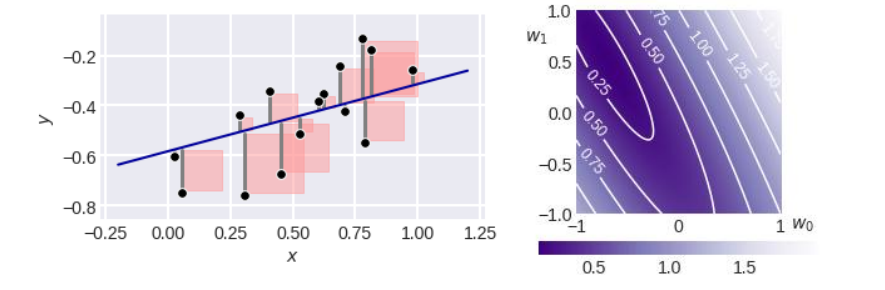
\includegraphics[scale=0.4]{pics/ml2_lin2.png}

Явное решение данной задачи:
$w_1 = \frac{\sum\limits_{i=1}^m (y_i - \overline y)(x_i - \overline x)}{\sum\limits_{i=1}^m (x_i - \overline x)^2} = \frac{cov(x_i, y_i)}{var(x_i)}$, $w_0 = \overline y - w_1 \overline x$, где $\overline x = \frac{1}{m} \sum\limits_{i=1}^m x_i$ и $\overline y = \frac{1}{m} \sum\limits_{i=1}^m y_i$

Общий случай $a(X_1, ..., X_n) = w_0 + w_1X_1 + ... + w_nX_n$:

Здесь $w = (w_0, w_1, ..., w_n)^T$ - вектор параметров (весов) линейной модели, а $x = (X_0, X_1, ..., X_n)^T$ – признаковое описание объекта. $X_0 \equiv 1$ - фиктивный признак.

Система уравнений:
\begin{equation*}
 \begin{cases}
   x_1^Tw = y_1,
   \\
   ...
   \\
   x_m^Tw = y_m
 \end{cases}
\end{equation*}

Или же $Xw = y$.

Задача оптимизации выглядит так $|| Xw - y ||_2^2 = \sum\limits_{i=1}^m (x_i^Tw - y_i)^2 \rightarrow min_w$

\begin{equation}
|| Xw - y ||_2^2 = (Xw - y)^T(Xw - y)= w^TX^TXw - w^TX^Ty - y^TXw +y^Ty
\end{equation}
\begin{equation}
\nabla || Xw - y ||_2^2 = 2X^TXw - 2X^Ty = 0
\end{equation}
\begin{equation}
 X^TXw = X^Ty
\end{equation}
\begin{equation}
 w = (X^TX)^{-1}X^Ty
\end{equation}
Решение существует, если столбцы матрицы X линейно независимы.
Матрица $(X^TX)^{-1}X^T$ называется псевдообратной матрицей Мура-Пенроуза.

Правило для запоминания: исходное матричное уравнение умножить на $X^T$ (слева и справа)

Обобщённая линейная регрессия $a(X_1, ..., X_n) = w_0 + w_1\phi_1(X_1, ..., X_n) + ... + w_k\phi_k(X_1, ..., X_n)$:
$\phi_1, ..., \phi_n$ - фиксированные базисные функции, не зависят от данных.

$a(x) = \sum\limits_{i=1}^k w_i\phi_i(x) = \phi(X)^Tw$ - решение.

$||\phi(X)^Tw - y||_2^2 \rightarrow min_w$ - задача оптимизации.

\subsubsection{Регуляризация}
В $(X^TX)^{-1}X^T$ происходит обращение матрицы которая может оказаться вырожденной. Эту проблему решает регуляризация.

Упрощённое объяснение её смысла в линейной модели
$a(X_1, ..., X_n) = w_0 + w_1X_1 + ... + w_nX_n$:
Если есть два похожих объекта, то должны быть похожи и их
метки. Пусть они отличаются в j-м признаке, тогда ответы модели отличаются
на $\epsilon_jw_j$. Поэтому не должно быть аномально больших по модулю весов
у признаков, по которым могут отличаться похожие объекты, а значит и у всех
признаков $X_1, ..., X_n$, поскольку заранее не известно, на каких объектах модель
будет работать. Заметим также, что константного признака это рассуждение не
касается.


Поэтому вместе с задачей
$|| Xw - y ||_2^2 \rightarrow min$
обычно стараются решить задачу
$|| w ||_2^2 = w_1^2 + ... + w_n^2 \rightarrow min$
(минимизации нормы весов).

Регуляризация Иванова:
\begin{equation*}
 \begin{cases}
   || Xw - y ||_2^2 \rightarrow min,
   \\
   || w ||_2^2 \leq \lambda
 \end{cases}
\end{equation*}

Регуляризация Тихонова (такой вид регуляризации называется также L2-регуляризацией):
\begin{equation*}
 \begin{cases}
   || Xw - y ||_2^2 + \lambda|| w ||_2^2 \rightarrow min,
   \\
   0 \leq \lambda
\end{cases}
\end{equation*}
Они эквивалентны. Решение указанной задачи регуляризации Тихонова задаётся формулой:
\begin{equation}\label{ss}
argmin(|| Xw - y ||_2^2 + \lambda|| w ||_2^2) = (X^TX + \lambda I)^{-1}X^Ty
\end{equation}
Для доказательства достаточно взять градиент и приравнять к нулю.

L1-регуляризация:
\begin{equation*}
 \begin{cases}
   \sum\limits_{i=1}^m (x_i^Tw - y_i)^2 + \lambda \sum\limits_{j=1}^n |w_j| \rightarrow min,
   \\
   0 \leq \lambda
\end{cases}
\end{equation*}

\subsubsection{Гребневая регрессия}
Регрессия с коэффициентами, определяемыми формулой \ref{ss} называется гребневой регрессией (Ridge Regression). Смысл гребневой регрессии – борьба с вырожденностью (плохой обусловленностью) матрицы $X^TX$. Коэффициент $\lambda$ называется коэффициентом регуляризации. При $\lambda = 0$ - классическое решение, при
$\lambda \rightarrow \infty$ матрица которую приходится обращать становится заведомо хорошо обусловленной, метод меньше «затачивается на данные».

Отметим, что для ridge-регрессии нужна правильная нормировка признаков
(как правило, стандартизация), при масштабировании (умножении признаков на
скаляры) результат может отличаться.

\subsubsection{Градиентный метод обучения}
На практике не применяется аналитическое решение. Для оптимизации $\frac{1}{2} \sum\limits_{i=1}^m (a(x_i|w) - y_i)^2 \rightarrow min$, где $a(x|w) = w^Tx$ используют итерационный метод (стохастический градиентный спуск):
\begin{equation}
w^{(t+1)} = w^{(t)} - n\nabla L_i(w^{(t)})
\end{equation}
\begin{equation}
w^{(t+1)} = w^{(t)} - n(a(x_i|w^{(t)}) - y_i)x_i
\end{equation}
Здесь $n$ - размер шага (скорость обучения).

\subsubsection{Линейные классификаторы}
Пусть $X= R^n$ и $Y = \{-1, 1\}$, рассмотрим линейную модель классификатора:
\begin{equation*}
a(x) = sgn(w^Tx + b) =
 \begin{cases}
   +1 &\text{, $w^Tx + b \geq 0$}\\
   -1 &\text{, $w^Tx + b < 0$}
 \end{cases}
\end{equation*}
Геометрический смысл линейного классификатора - пространство делится гиперплоскостью на два полупространства:

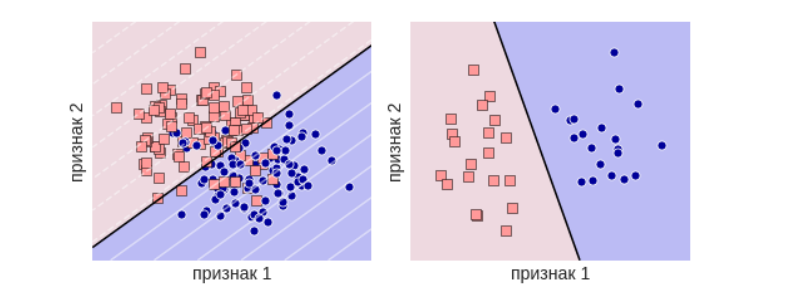
\includegraphics[scale=0.4]{pics/ml2_lin3.png}

При обучении минимизируем число ошибок:
\begin{equation}
L(X_{train}, a) = \sum\limits_{t=1}^m L(y_t, a(x_t)) \rightarrow min
\end{equation}
\begin{equation*}
L(y_t, a(x_t)) =
 \begin{cases}
   1 &\text{, $sgn(w^Tx_t) = y_t'$, $y'$ - элемент отображения $Y = \{-1, 1\}$ на $Y' = \{0, 1\}$}\\
   0 &\text{, $sgn(w^Tx_t) \ne y_t'$}
 \end{cases}
\end{equation*}

\subsubsection{Метод опорных векторов}
Перейдем к системе вида:
\begin{equation*}
a(x) = sgn(w^Tx + b) =
 \begin{cases}
   +1 &\text{, $w^Tx + b \geq 1$}\\
   -1 &\text{, $w^Tx + b \leq -1$}
 \end{cases}
\end{equation*}
Такой переход возможен за счет выполнения равенства $sgn(w^Tx + b) = sgn(\alpha w^Tx + \alpha b), \alpha > 0$ приводящему к $y_i(w^Tx_i + b) > 1$, считаем что $min_i|w^Tx_i + b| = 1$.

Расстояние от $x_i$ до гиперплоскости $w^Tx + b = 0$ равно $p(x_i, w^Tx + b) = \frac{|w^Tx_i + b|}{||w||}$.

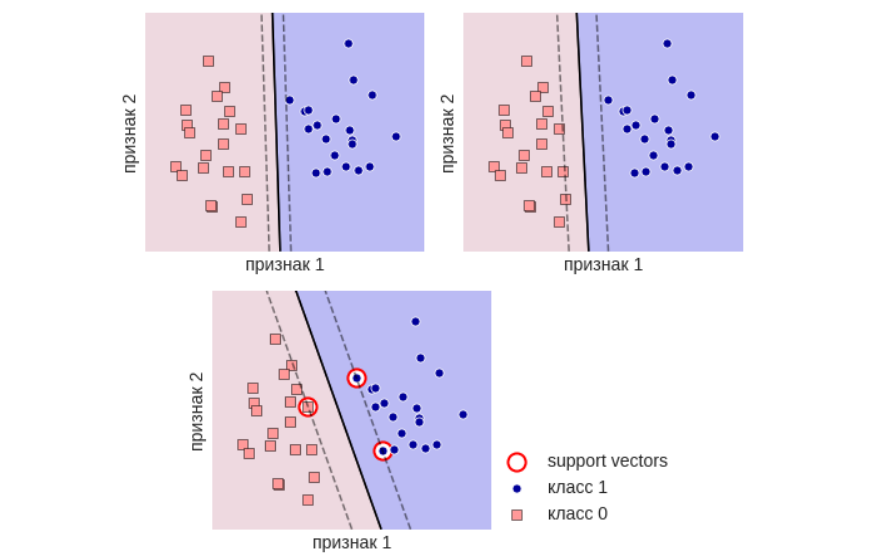
\includegraphics[scale=0.4]{pics/ml2_lin4.png}

Максимизируем минимум из этих расстояний (зазор):
\begin{equation}
min_i\frac{|w^Tx_i + b|}{||w||} = \frac{1}{||w||} \rightarrow max
\end{equation}

Можно перейти к задаче квадратичного программирования с m ограничениями:
\begin{equation}
y_i(w^Tx_i + b) > 1, i=\overline{1,m}
\end{equation}
\begin{equation}
\frac{||w||^2}{2} \rightarrow min
\end{equation}
А далее уже как обычно решаем задачу оптимизации, Лагранжиан там, бла-бла-бла...

Краткое описание решения:
\begin{enumerate}
    \item Построить матрицу $H = || y_iy_jx_i^Tx_j ||_{m * m}$
    \item Решить задачу оптимизации $-\frac{1}{2}\alpha^TH\alpha + \overline{1}^T\alpha \rightarrow max$ при условиях $\alpha \geq 0$ и $y^T\alpha = 0$
    \item Выразить параметры метода:
    \begin{equation}
    w = \sum\limits_{i=1}^m \alpha_iy_ix_i
    \end{equation}
    \begin{equation}
    S = \{i \in \{1,2,3,...,m\} | \alpha_i > 0\}
    \end{equation}
    \begin{equation}
    b = \frac{1}{|S|}\sum\limits_{i \in S} (y_i - w^Tx_i) = \frac{1}{|S|}\sum\limits_{i \in S} (y_i - \sum\limits_{i \in S}\alpha_j y_jx_j^Tx_i)
    \end{equation}
\end{enumerate}

Итоговое решение имеет вид $a(x) = sgn(w^Tx + b) = sgn(\sum\limits_{i \in S} \alpha_i y_ix_i^Tx + b)$

SVM довольно чувствителен к масштабированию признаков и наличию шумовых признаков.
